\documentclass[preview,tikz]{standalone}
\usepackage{amssymb,amsmath,amsthm,amsfonts}
\usepackage{listings}
\usepackage{tikz}

\usetikzlibrary{calc}
\usetikzlibrary{decorations.pathreplacing}
\usetikzlibrary{fit}
\usetikzlibrary{patterns.meta}
\usetikzlibrary{shapes.geometric}

% Custom colors
\usepackage{color}
\definecolor{deepblue}{rgb}{0,0,0.5}
\definecolor{deepred}{rgb}{0.6,0,0}
\definecolor{deepgreen}{rgb}{0,0.5,0}

% Python style for highlighting
\lstset{
    language=Python,
    basicstyle=\small\ttfamily,
    morekeywords={self, max, min, float},              % Add keywords here
    keywordstyle=\color{deepblue},
    emph={
        __init__,
        __getitem__,
    },          % Custom highlighting
    emphstyle=\color{deepred},    % Custom highlighting style
    stringstyle=\color{deepgreen},
    frame=tb,                         % Any extra options here
    showstringspaces=false,
}

\begin{document}
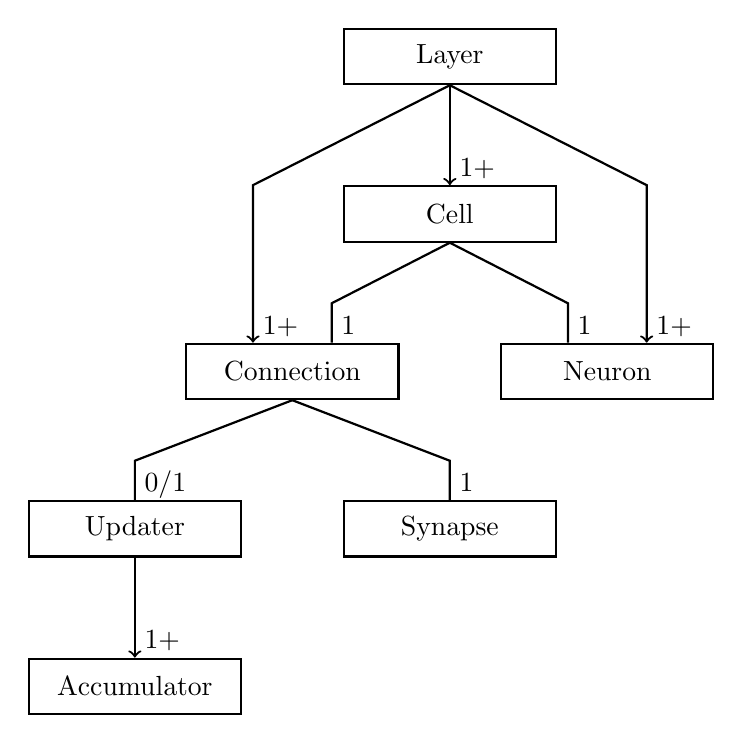
\begin{tikzpicture}[
    component/.style ={rectangle, draw=black, thick, fill=none, text width=7em, text centered, minimum height=2em},
    arity/.style ={rectangle, draw=none, fill=none, align=left, text height=1em, text depth=0.1em},
]
    % components
    \node[component] (layer) at (0,0) {\lstinline|Layer|};
    \node[component] (cell) at (0,-2) {\lstinline|Cell|};
    \node[component] (conn) at (-2,-4) {\lstinline|Connection|};
    \node[component] (neur) at (2,-4) {\lstinline|Neuron|};
    \node[component] (syn) at (0,-6) {\lstinline|Synapse|};
    \node[component] (updater) at (-4,-6) {\lstinline|Updater|};
    \node[component] (acc) at (-4,-8) {\lstinline|Accumulator|};

    %arity labels
    \node[arity, anchor=south west] (lcell) at ($(cell.north) - (0, 0.05)$) {1+};
    \node[arity, anchor=south west] (lc) at ($(conn.north) - (0.5, 0) - (0, 0.05)$) {1+};
    \node[arity, anchor=south west] (cc) at ($(conn.north) + (0.5, 0) - (0, 0.05)$) {1};
    \node[arity, anchor=south west] (ln) at ($(neur.north) + (0.5, 0) - (0, 0.05)$) {1+};
    \node[arity, anchor=south west] (cn) at ($(neur.north) - (0.5, 0) - (0, 0.05)$) {1};
    \node[arity, anchor=south west] (cu) at ($(updater.north) - (0, 0.05)$) {0/1};
    \node[arity, anchor=south west] (cs) at ($(syn.north) - (0, 0.05)$) {1};
    \node[arity, anchor=south west] (ua) at ($(acc.north) - (0, 0.05)$) {1+};

    % edges
    \draw[->, thick] (layer) edge[thick] (cell);
    \draw[->, thick] (layer.south) -- ($(-2.5, 0) + (cell.north)$) -- ($(conn.north) - (0.5, 0)$);
    \draw[->, thick] (layer.south) -- ($(2.5, 0) + (cell.north)$) -- ($(neur.north) + (0.5, 0)$);
    \draw[thick] (cell.south) -- ($(conn.north) + (0.5, 0.5)$) -- ($(conn.north) + (0.5, 0)$);
    \draw[thick] (cell.south) -- ($(neur.north) + (-0.5, 0.5)$) -- ($(neur.north) - (0.5, 0)$);
    \draw[thick] (conn.south) -- ($(updater.north) + (0, 0.5)$) -- (updater.north);
    \draw[thick] (conn.south) -- ($(syn.north) + (0, 0.5)$) -- (syn.north);
    \draw[->, thick] (updater.south) -- (acc.north);
\end{tikzpicture}
\end{document}